\section{绝对值函数}
\begin{definition}[绝对值]
设\(x \in \mathbb{R}\),则称函数\[
	f(x) = \left\{ \begin{array}{c}
		x, \quad x \geq 0 \\
		-x, \quad x < 0
	\end{array} \right.
\]为\(x\)的绝对值,
记作\(\abs{x}\).
\end{definition}

\begin{figure}[ht]
	\centering
	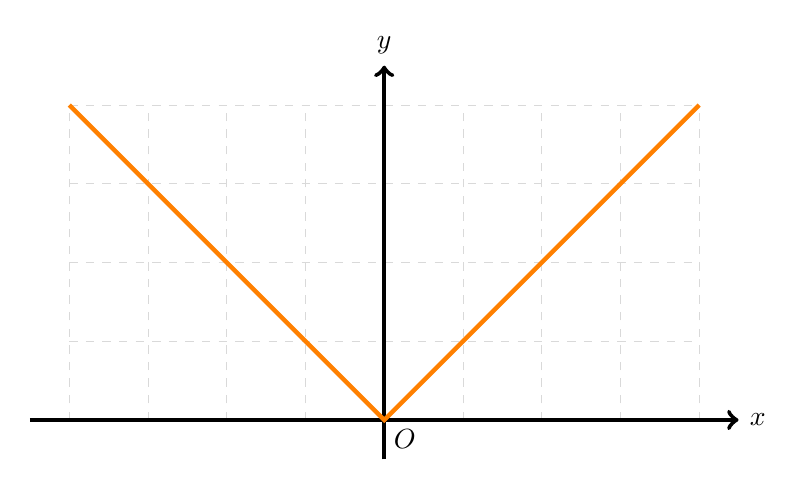
\begin{tikzpicture}
		\draw[help lines, color=gray!30, dashed] (-4,0) grid (4,4);
		\draw[->, ultra thick] (-4.5,0) -- (4.5,0) node[right]{\(x\)};
		\draw[->, ultra thick] (0,-0.5) -- (0,4.5) node[above]{\(y\)};
		\draw (0,0)node[below right]{\(O\)};
		\draw[orange,ultra thick] (-4,4)--(0,0)--(4,4);
	\end{tikzpicture}
	\caption{绝对值函数\(\abs{x}\)的图形}
\end{figure}

\begin{gather}
	\min\{a,b\}
	= \frac{a+b}{2}
	- \frac{\abs{a-b}}{2}, \\
	\max\{a,b\}
	= \frac{a+b}{2}
	+ \frac{\abs{a-b}}{2}.
\end{gather}
